\documentclass[journal,10pt,twoside]{IEEEtran}

% ---------- Packages ----------
\usepackage{amsmath,amssymb,amsthm}
\usepackage{mathtools}
\usepackage{algorithm}
\usepackage[noend]{algpseudocode}
\usepackage{booktabs}
\usepackage{array}
\usepackage{multirow}
\usepackage{url}
\usepackage{cite}
\usepackage{microtype}
\usepackage{xcolor}
\usepackage{pifont}
\usepackage{amssymb}
\DeclareMathOperator{\rank}{rank}
\DeclareMathOperator{\sel}{sel}
\usepackage{tikz}
\usetikzlibrary{positioning,arrows.meta,shapes.geometric,
                fit,backgrounds,calc}

% ---------- Colours ----------
\definecolor{colA}{RGB}{22,114,91}
\definecolor{colB}{RGB}{30,90,165}
\definecolor{colC}{RGB}{120,50,180}
\definecolor{colD}{RGB}{190,100,10}
\definecolor{colE}{RGB}{170,35,35}
\definecolor{lightgray}{RGB}{240,240,240}

% ---------- Check / cross marks ----------
\newcommand{\cmark}{\ding{51}}
\newcommand{\xmark}{\ding{55}}

% ---------- Theorem environments ----------
\newtheorem{theorem}{Theorem}[section]
\newtheorem{lemma}[theorem]{Lemma}
\newtheorem{corollary}[theorem]{Corollary}
\newtheorem{proposition}[theorem]{Proposition}
\newtheorem{definition}[theorem]{Definition}
\newtheorem{invariant}{Invariant}[section]
\newtheorem{remark}{Remark}[section]

% ---------- Notation ----------
\newcommand{\SCPG}{\mathcal{G}}
\newcommand{\VT}{V_{\!\mathrm{tok}}}
\newcommand{\VS}{V_{\!\mathrm{syn}}}
\newcommand{\VB}{V_{\!\mathrm{bb}}}
\newcommand{\VSSA}{V_{\!\mathrm{ssa}}}
\newcommand{\VSYM}{V_{\!\mathrm{sym}}}
\newcommand{\EAST}{E^{\mathrm{AST}}}
\newcommand{\ECFG}{E^{\mathrm{CFG}}}
\newcommand{\EDFG}{E^{\mathrm{DFG}}}
\newcommand{\ECDG}{E^{\mathrm{CDG}}}
\newcommand{\ECG}{E^{\mathrm{CG}}}
\newcommand{\ETH}{E^{\mathrm{TH}}}
\newcommand{\SigN}{\Sigma_{\!N}}
\newcommand{\SigE}{\Sigma_{\!E}}
\newcommand{\SigPhi}{\Sigma_{\!\Phi}}
\newcommand{\tauF}{\tau}
\newcommand{\tauI}{\tau^{-1}}
\newcommand{\FI}{\mathcal{FI}}
\newcommand{\BI}{\mathcal{BI}}
\newcommand{\ROBDD}{\mathrm{ROBDD}}
\newcommand{\SATC}{\#\mathrm{SAT}}
\newcommand{\DF}{\mathrm{DF}}
\newcommand{\idom}{\mathrm{idom}}
\newcommand{\BigO}{\mathcal{O}}
\newcommand{\sortkey}{\mathit{skey}}
\newcommand{\pre}{\mathrm{pre}}
\newcommand{\hscpg}{h_{\mathrm{scpg}}}

% ============================================================
\begin{document}

\title{OpenHeart: A Succinct Compositional Program Graph\\
for Polynomial-Time Universal Program Analysis\\
and UML Visualization}

\author{%
\IEEEauthorblockN{[Author Names Redacted for Review]}\\
\IEEEauthorblockA{[Affiliations Redacted for Review]}}

\maketitle

% ============================================================
\begin{abstract}
Program analysis tools have long suffered from
\textit{representational fragmentation}: compiler frameworks
discard the high-level semantics needed for visualization,
while modeling tools lack the analytical power required for
dataflow analysis.  No single intermediate representation
today simultaneously supports UML diagram generation,
bidirectional source navigation, interprocedural dataflow,
and path-coverage analysis---all with provable efficiency.

We present the \textbf{Succinct Compositional Program Graph
(SCPG)} and the \textbf{OpenHeart} ten-phase construction
pipeline.  The SCPG is a unified data structure that encodes
a codebase's complete semantic content---from raw tokens to
UML behavioral metadata---within one memory-mapped binary
artifact.  We define four formal requirements on a universal
program representation (space efficiency, total traceability,
UML completeness, polynomial queries) and prove the SCPG
satisfies all four.  Key results include: $\BigO(n\log\sigma)$-bit
storage via Balanced Parentheses encoding and Wavelet Trees;
$\BigO(1)$ backward and $\BigO(\log n)$ forward source
navigation; per-function path summaries of size $\BigO(m)$
for structured programs via a novel structural induction;
and $\BigO(|N|\cdot|D|^2)$ interprocedural dataflow via IFDS.
We prove that the Code Property Graph, LLVM IR, and EMF/XMI
each violate at least one requirement, establishing the SCPG
as strictly more capable than any single predecessor.
\end{abstract}

\begin{IEEEkeywords}
Program analysis, succinct data structures, static single
assignment, binary decision diagrams, UML generation,
code property graphs, interprocedural dataflow, traceability.
\end{IEEEkeywords}

% ============================================================
\section{Introduction}\label{sec:intro}

\subsection{The Problem}

Consider a senior engineer responsible for auditing a
production payment service written in Java.  She has four
simultaneous needs.  First, she wants a UML class diagram of
the service layer to communicate its structure to
stakeholders---with every class box clickable, jumping
directly to the corresponding source declaration.  Second, she
needs a sequence diagram showing the call chain from
\texttt{processOrder} to the database layer, so she can
identify which messages cross trust boundaries.  Third, she
needs a taint analysis that proves no unvalidated user input
reaches a SQL query.  Fourth, her team's CI pipeline must
regenerate all of these artifacts automatically whenever a
developer commits a change, in under two seconds.

In practice, she cannot satisfy all four needs with any single
tool.  LLVM IR~\cite{lattner04} handles the taint analysis but
discards class hierarchies during lowering, making UML
generation impossible.  Joern~\cite{yamaguchi14} preserves
structural information in a Code Property Graph (CPG) but
stores it in a graph database with $7$--$35\times$ overhead
and provides no formal traceability guarantee between diagram
elements and source tokens.  EMF/XMI~\cite{emf} generates
UML models but provides no built-in graph analysis.  Each
tool requires a separate import/export cycle, and none
guarantees that a UML element's source location is accurate
after a code edit.

\subsection{Our Approach}

This paper introduces the \textit{Succinct Compositional
Program Graph} (SCPG) and the \textit{OpenHeart} pipeline,
which close this gap with a single, formally specified
representation.  The core insight is that the five
analytically distinct layers of a program---lexical tokens,
abstract syntax, control flow, data flow, and declared
symbols---can be unified within one data structure that is
simultaneously space-optimal, fully traceable, semantically
complete for UML, and analytically powerful.

The SCPG's design rests on four techniques from the
foundations of computer science: (1) \textit{Balanced
Parentheses encoding}~\cite{munroraman97,sadakanenavarro14}
for the AST, achieving $2n + o(n)$ bits with $\BigO(1)$
navigation; (2) \textit{Wavelet Trees}~\cite{grossi03} for
typed edge labels, enabling $\BigO(\log\sigma)$ type-filtered
traversal at $\lceil\log_2\sigma\rceil$ bits per edge;
(3) \textit{SSA form}~\cite{cytron91} for the data-flow
layer, making every def-use relationship explicit and
queryable in $\BigO(1)$; and (4) \textit{Reduced Ordered
BDDs}~\cite{bryant86} for per-function path summaries,
encoding exponentially many paths in polynomial space for
structured programs.

\subsection{Contributions}

We make the following specific contributions:

\begin{enumerate}
\item We define four axiomatic requirements (\textbf{R1--R4})
  on a universal program representation
  (Section~\ref{sec:problem}) and prove the SCPG satisfies
  all four.

\item We introduce the SCPG formally as a seven-tuple
  $\SCPG = (V, E, \nu, \varepsilon, \tauF, \rho, \SigPhi)$
  and prove that it stores a codebase in
  $\BigO(n\log\sigma)$ bits (Section~\ref{sec:model}).

\item We prove the \textit{Traceability Completeness Theorem}:
  every SCPG entity has a well-defined source range, and the
  inverse query is answerable in $\BigO(\log n)$
  (Section~\ref{sec:theory}).

\item We prove by structural induction that for any
  series-parallel CFG, the ROBDD encoding of the feasible
  path function has at most $2m-1$ nodes
  (Section~\ref{sec:theory}).  This proof does not require
  treewidth machinery and follows directly from the CFG's
  recursive structure.

\item We define the UMLLink record and the SCPG hash chain
  (Section~\ref{sec:model}), enabling stale-diagram
  detection in $\BigO(1)$ after any source edit.

\item We prove that the Code Property
  Graph~\cite{yamaguchi14}, LLVM IR~\cite{lattner04}, and
  EMF/XMI~\cite{emf} each violate at least one of R1--R4
  (Section~\ref{sec:comparison}).
\end{enumerate}

\paragraph{Scope.}
This paper presents the SCPG as a formal framework with
analytical complexity bounds.  Empirical evaluation on
industrial codebases is planned future work.

% ============================================================
\section{Requirements and Baseline Comparison}
\label{sec:problem}

Before defining the SCPG, we state the four requirements that
any universal program representation must satisfy.  These
requirements are not aspirational---each is directly necessary
for at least one of the use cases in the introduction.

\begin{description}
\item[\textbf{R1 (Space Efficiency).}] Storage in
  $\BigO(n\log\sigma)$ bits, where $n = |V| + |E|$ is the
  total entity count and $\sigma = |\SigN| + |\SigE| \le 256$
  is the combined node/edge type alphabet size.  This is
  within a logarithmic factor of the information-theoretic
  minimum for typed graphs.

\item[\textbf{R2 (Absolute Traceability).}] A total,
  invertible function $\tauF : \mathcal{E} \to \mathcal{R}$
  mapping every IR entity to its source text range, with
  $\BigO(1)$ backward evaluation (entity $\to$ range) and
  $\BigO(\log n)$ forward evaluation (position $\to$ entity
  set), plus a formally provable roundtrip property.

\item[\textbf{R3 (Semantic Completeness).}] Sufficient
  metadata to derive all fourteen UML~2.5
  diagram types~\cite{uml25} in polynomial time from the
  representation alone.

\item[\textbf{R4 (Polynomial Query Complexity).}]
  Interprocedural dataflow, path reachability, program
  slicing, and test coverage answerable in polynomial time
  with formal worst-case bounds.
\end{description}

Table~\ref{tab:compare} evaluates five systems against these
requirements.  No predecessor satisfies all four; the SCPG
does.  We prove these violations formally in
Section~\ref{sec:comparison}.

\begin{table}[!t]
\renewcommand{\arraystretch}{1.3}
\caption{Satisfaction of Requirements R1--R4}
\label{tab:compare}
\centering
\small
\begin{tabular}{@{}lcccc@{}}
\toprule
\textbf{System} & \textbf{R1} & \textbf{R2} &
  \textbf{R3} & \textbf{R4}\\
\midrule
CPG / Joern~\cite{yamaguchi14}  & \xmark & \xmark & \xmark & \cmark\\
LLVM IR~\cite{lattner04}         & \cmark & \xmark & \xmark & \cmark\\
EMF / XMI~\cite{emf}             & \xmark & \xmark & partial & \xmark\\
WALA~\cite{wala}                 & \xmark & partial & \xmark & \cmark\\
\textbf{SCPG (OpenHeart)}        & \cmark & \cmark & \cmark & \cmark\\
\bottomrule
\end{tabular}
\end{table}

% ============================================================
\section{Background}\label{sec:background}

This section introduces the three foundational techniques
on which the SCPG rests.  Readers familiar with succinct data
structures, SSA form, and binary decision diagrams may skip
to Section~\ref{sec:model}.

\subsection{Succinct Tree Encoding}

An ordered tree on $n$ nodes can be stored naively with four
pointer-sized fields per node ($\sim 32$ bytes), totaling
$32n$ bytes.  Yet the information-theoretic lower bound is
only $2n - \BigO(\log n)$ bits---a factor-of-$128$ gap for
32-bit nodes.

The \textit{Balanced Parentheses (BP) encoding} closes this
gap.  A DFS traversal emits a $1$-bit (``open'') at each
pre-order visit and a $0$-bit (``close'') at each
post-order backtrack.  The resulting binary string has length
$2n$ and encodes the complete tree structure.  Augmenting it
with a $o(n)$-bit \textit{rank-select index}---which supports
$\rank_1(i) = |\{j \le i : B[j]=1\}|$ and its inverse
$\sel_1(j)$ in $\BigO(1)$---enables all standard navigation
operations ($\mathrm{parent}$, $\mathrm{first\_child}$,
$\mathrm{next\_sibling}$, $\mathrm{LCA}$, $\mathrm{depth}$)
to execute in $\BigO(1)$ time~\cite{munroraman97,
sadakanenavarro14}.

A closely related structure, the \textit{Wavelet
Tree}~\cite{grossi03}, provides $\BigO(\log\sigma)$-time
access, rank, and select operations over a sequence of
length $m$ drawn from an alphabet of size $\sigma$, using
$m\lceil\log_2\sigma\rceil + \BigO(m)$ bits.  In the SCPG,
a Wavelet Tree encodes the edge type of every adjacency-list
entry, enabling $\BigO(\log\sigma)$ type-filtered graph
traversal without maintaining separate per-type adjacency
lists.

\subsection{Static Single Assignment Form}

Program analysis becomes dramatically simpler when every
variable has exactly one definition site.  Static Single
Assignment (SSA) form~\cite{cytron91} guarantees this by
renaming each source variable $v$ into a set of versions
$\{v^0, v^1, \ldots\}$, one per definition.  At control-flow
join points (blocks with $\ge 2$ predecessors), $\phi$-functions
of the form $v^r = \phi(v^{a_1},\ldots,v^{a_p})$ select the
correct reaching definition.  A key property: given any use
of $v^k$, its unique definition is found in $\BigO(1)$ by
array lookup, making all dataflow edges explicit and sparse.

Cytron et al.~\cite{cytron91} showed that $\phi$-functions
need only be placed at the \textit{iterated dominance frontier}
of each variable's definition sites.  The total number of
$\phi$-insertions across all variables in a function is
$\BigO(|E_{\mathrm{cfg}}|)$---proportional to the number of
CFG edges, not the number of variables.

\subsection{Binary Decision Diagrams for Path Analysis}

A function with $k$ independent binary branches has up to
$2^k$ distinct execution paths.  For $k = 40$, direct
enumeration is intractable.  \textit{Reduced Ordered BDDs
(ROBDDs)}~\cite{bryant86} represent Boolean functions over
path-indicator variables as maximally shared DAGs.  Two
reduction rules---eliminating nodes whose branches are
identical (R1) and merging isomorphic subgraphs (R2)---yield
a canonical representation whose size depends on the
structure of the underlying graph, not the number of paths.
For the class of \textit{series-parallel} CFGs (which
includes all structured programs), we prove in
Section~\ref{sec:theory} that the ROBDD has size $\BigO(m)$
where $m = |E_{\mathrm{cfg}}|$.

The \textit{IFDS framework}~\cite{reps95} solves the
complementary problem: given a family of dataflow facts $D$
and \textit{distributive} flow functions ($f(X \cup Y) =
f(X) \cup f(Y)$), the precise interprocedural solution is
computable in $\BigO(|N| \cdot |D|^2)$ time.  Taint analysis,
null checking, and type-state validation all fit this model.

% ============================================================
\section{The SCPG Formal Model}\label{sec:model}

\subsection{Vertex Layers and the Seven-Tuple}

The SCPG organizes a codebase's entities into five
semantically distinct \textit{layers}.  Think of these layers
as a vertical stack: at the bottom sit the raw source tokens;
above them, the abstract syntax tree; then the control flow
graph's basic blocks; then the SSA variables; and at the top,
the declared symbols (classes, methods, fields).  Crucially,
this is not five separate data structures---it is one unified
hypergraph in which every entity at every layer has a direct
pointer to its originating source token, enabling navigation
in any direction.

\begin{definition}[SCPG]\label{def:scpg}
A \emph{Succinct Compositional Program Graph} is a seven-tuple
\[
  \SCPG = (V,\; E,\; \nu,\; \varepsilon,\; \tauF,\;
           \rho,\; \SigPhi)
\]
with the following components.

\smallskip\noindent\textbf{Vertices.}
$V = \VT \uplus \VS \uplus \VB \uplus \VSSA \uplus \VSYM$
is a disjoint union of five layers:
$\VT$ (one vertex per source lexeme),
$\VS$ (AST internal nodes),
$\VB$ (basic blocks in all functions),
$\VSSA$ (SSA variable definition sites),
$\VSYM$ (declared symbols: classes, interfaces, methods,
fields).

\smallskip\noindent\textbf{Edges.}
$E \subseteq V \times V \times \SigE$ decomposes as
$E = \EAST \cup \ECFG \cup \EDFG \cup \ECDG \cup
     \ECG \cup \ETH$
(AST parent-child, control flow, data flow/def-use, control
dependence, call graph, and type hierarchy).

\smallskip\noindent\textbf{Node typing.}
$\nu : V \to \SigN \times (\mathrm{Attr} \to \mathrm{Val})^*$
assigns each vertex a type from the finite alphabet $\SigN$
and a property map.

\smallskip\noindent\textbf{Edge typing.}
$\varepsilon : E \to \SigE$ assigns each edge a type from
the finite alphabet $\SigE$, with $|\SigE| \le 16$ in
standard deployment.

\smallskip\noindent\textbf{Source location.}
$\tauF : \VT \to \mathbb{N}^4$ maps each token vertex to
$(\mathit{file}, \mathit{line}, \mathit{col}, \mathit{len})$.
This is the ground truth for all traceability.

\smallskip\noindent\textbf{UML metadata.}
$\rho : \VSYM \to \mathcal{M}$ assigns UML rendering
metadata to each symbol vertex.

\smallskip\noindent\textbf{Path summaries.}
$\SigPhi : \{f \in \VSYM : \nu(f).\mathit{kind} =
\mathrm{FUNC}\} \to \ROBDD$ maps each function symbol to a
Reduced Ordered BDD encoding its feasible execution paths.
\end{definition}

Figure~\ref{fig:layers} illustrates the layer structure.

\begin{figure}[!t]
\centering
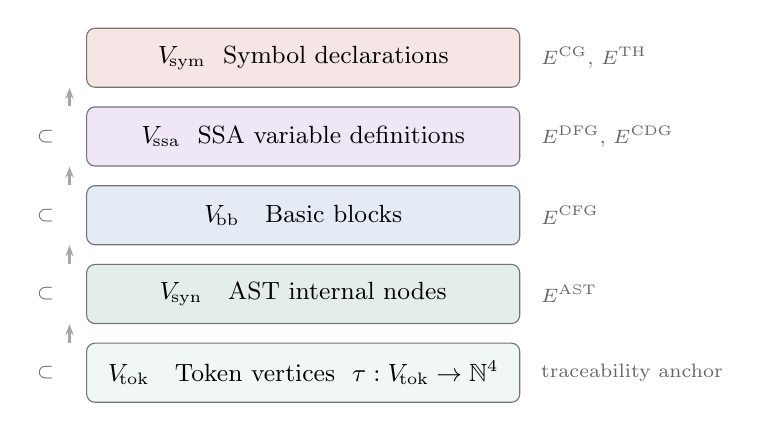
\begin{tikzpicture}[
  box/.style={
    draw=black!55, rounded corners=3pt,
    minimum width=5.5cm, minimum height=0.75cm,
    font=\small, align=left, inner sep=4pt
  },
  lbl/.style={font=\scriptsize, text=black!60},
  arr/.style={-{Stealth[length=4pt]},thick,black!35}
]

\node[box, fill=colE!12] (sym) at (0,4.0)
  {\textbf{$\VSYM$}\ \ Symbol declarations};
\node[box, fill=colC!12] (ssa) at (0,3.0)
  {\textbf{$\VSSA$}\ \ SSA variable definitions};
\node[box, fill=colB!12] (bb)  at (0,2.0)
  {\textbf{$\VB$}\ \ \ Basic blocks};
\node[box, fill=colA!12] (syn) at (0,1.0)
  {\textbf{$\VS$}\ \ \ AST internal nodes};
\node[box, fill=colA!6]  (tok) at (0,0.0)
  {\textbf{$\VT$}\ \ \ Token vertices\ \ $\tauF : \VT \to \mathbb{N}^4$};

\draw[arr] ([xshift=-6pt]tok.north west)
  -- ([xshift=-6pt]syn.south west);
\draw[arr] ([xshift=-6pt]syn.north west)
  -- ([xshift=-6pt]bb.south west);
\draw[arr] ([xshift=-6pt]bb.north west)
  -- ([xshift=-6pt]ssa.south west);
\draw[arr] ([xshift=-6pt]ssa.north west)
  -- ([xshift=-6pt]sym.south west);

\node[lbl,left=8pt of tok.west,anchor=east]
  {$\subset$};
\node[lbl,left=8pt of syn.west,anchor=east]
  {$\subset$};
\node[lbl,left=8pt of bb.west,anchor=east]
  {$\subset$};
\node[lbl,left=8pt of ssa.west,anchor=east]
  {$\subset$};

\node[lbl,right=4pt of sym.east,anchor=west]
  {$\ECG$, $\ETH$};
\node[lbl,right=4pt of ssa.east,anchor=west]
  {$\EDFG$, $\ECDG$};
\node[lbl,right=4pt of bb.east,anchor=west]
  {$\ECFG$};
\node[lbl,right=4pt of syn.east,anchor=west]
  {$\EAST$};
\node[lbl,right=4pt of tok.east,anchor=west]
  {traceability anchor};

\end{tikzpicture}
\caption{The five vertex layers of the SCPG.  The subsumption
arrows ($\subset$) indicate that each layer's entities are
anchored in the layers below: every AST node spans a contiguous
token range; every basic block corresponds to a statement
sub-sequence; every SSA variable traces to a defining
statement.  The token layer is the traceability ground truth:
$\tauF$ is defined here and propagated upward by Phase~2.}
\label{fig:layers}
\end{figure}

\subsection{Source Position Encoding}

Every token vertex is assigned a $64$-bit \textit{sort key}
that encodes its file, line, and column:
\begin{equation}\label{eq:sortkey}
\sortkey(\mathit{file}, \ell, c)
  = (\mathit{file} \ll 48) \mid (\ell \ll 24)
    \mid (c \ll 8).
\end{equation}
This packing is injective (bit fields are non-overlapping
and individually bounded), so distinct source positions
yield distinct sort keys.  Sorting token records by
$\sortkey$ creates the \textit{forward index} $\FI$,
enabling $\BigO(\log n_t)$ source-position-to-token lookup.
The complementary \textit{backward index} $\BI$ is a
dense array indexed by token identifier, giving $\BigO(1)$
token-to-source-position lookup.

\subsection{The Traceability Layer}

Every entity at every layer is pinned to a source range
via the backward traceability function.

\begin{definition}[Backward Traceability Function]\label{def:tau}
Let $\mathcal{E} = \{L_0, \ldots, L_5\} \times \mathbb{N}$
be the set of all entity references, where $L_0, \ldots, L_5$
denote the token, AST, symbol, block, SSA, and call-site
layers respectively.  The function
$\tauF : \mathcal{E} \to \mathcal{R}$, where $\mathcal{R}$
is the set of source ranges, is defined by:
\begin{align}
  \tauF(L_0, t) &= \mathrm{point}(\BI[t])
  \label{eq:tau0}\\
  \tauF(L_1, v) &= \mathrm{span}(\BI[\mathit{ft}(v)],
    \BI[\mathit{lt}(v)])
  \label{eq:tau1}\\
  \tauF(L_2, s) &= \tauF(L_1, \mathit{decl}(s))
  \label{eq:tau2}\\
  \tauF(L_3, b) &= \mathrm{span}(\BI[\mathit{fbt}(b)],
    \BI[\mathit{lbt}(b)])
  \label{eq:tau3}\\
  \tauF(L_4, v) &= \tauF(L_1, \mathit{def\_stmt}(v))
  \label{eq:tau4}\\
  \tauF(L_5, c) &= \tauF(L_0, \mathit{call\_tok}(c))
  \label{eq:tau5}
\end{align}
where $\mathit{ft}(v)$/$\mathit{lt}(v)$ are the first/last
token indices in the subtree of AST node $v$, propagated
bottom-up during Phase~2.
\end{definition}

The \textit{Symbol Span Index} $\FI$ is an array of records
$(\mathit{ft}, \mathit{lt}, \mathit{sym\_id},
\mathit{file})$ sorted by $(\mathit{file}, \mathit{ft})$.
It enables the \textit{forward traceability query}:
\[
  \tauI(\mathit{file}, t) =
  \{r.\mathit{sym\_id} : r.\mathit{ft} \le t
    \le r.\mathit{lt}\}
\]
answerable in $\BigO(\log n_s + k)$ by binary search
followed by a backward scan, where $k$ is the result size.

\smallskip
Every UML diagram element carries a \textit{UMLLink
record}---a 24-byte structure embedding the source range
$\tauF(L_2, s)$ and a \textit{composite SCPG hash}:
\begin{equation}\label{eq:hashchain}
  \hscpg = \mathrm{CRC32}(h_1 \oplus h_2 \oplus \cdots
  \oplus h_6)
\end{equation}
where $h_i = \mathrm{CRC64}(\mathit{bytes}(A_i))$
for each of the six upstream pipeline artifacts.  Any source
edit changes at least one $h_i$ with probability
$1 - 2^{-64}$, changing $\hscpg$ and rendering affected
UMLLinks stale---detectable in $\BigO(1)$ by a single
integer comparison.

% ============================================================
\section{The OpenHeart Construction Pipeline}\label{sec:pipeline}

OpenHeart constructs the SCPG through ten sequential phases.
Each phase is a total function
$\Phi_i : \mathcal{A}_i \to \mathcal{A}_{i+1}$ that reads
a set of immutable artifacts and emits exactly one new
immutable artifact.  Table~\ref{tab:pipeline} lists the
phases with their output artifact, dominant time complexity,
and uncompressed output size for a representative 500K-LOC
Java project.  Figure~\ref{fig:pipeline} shows the
data-flow between phases.

\begin{table}[!t]
\renewcommand{\arraystretch}{1.25}
\caption{The Ten-Phase OpenHeart Pipeline}
\label{tab:pipeline}
\centering
\small
\begin{tabular}{@{}c@{\,}l@{\;}l@{\;}r@{}}
\toprule
\textbf{Ph.} & \textbf{Name} & \textbf{Cost}
  & \textbf{Size}\\
\midrule
1  & Lexical Ingestion   & $\BigO(N + n_t\log n_t)$  & 37\,MB\\
2  & BP AST Encoding     & $\BigO(n_a\log n_a)$      & 45\,MB\\
3  & Symbol Table        & $\BigO(n_a)$              &  9\,MB\\
4  & CFG + Dominators    & $\BigO(n_a + \Sigma n_b^2)$&27\,MB\\
5  & SSA + IFDS          & $\BigO(n_a|D|^2)$         &105\,MB\\
6  & Call Graph          & $\BigO(n_p^{1.5})$        &  8\,MB\\
7  & Traceability Index  & $\BigO(n_s\log n_s)$      & 39\,MB\\
8  & ROBDD Path Summaries& $\BigO(m|\ROBDD|n_f)$     & 92\,MB\\
9  & UML Extraction      & $\BigO(n_a + n_c P)$      & 15\,MB\\
10 & SCPG Assembly       & $\BigO(A_{\mathrm{tot}})$ & 82\,MB\textsuperscript{*}\\
\bottomrule
\multicolumn{4}{l}{\scriptsize\textsuperscript{*}LZ4-compressed.
  $N$: source bytes; $n_t$: tokens; $n_a$: AST nodes;}\\
\multicolumn{4}{l}{\scriptsize $n_s$: symbols; $n_p$: pointer vars;
  $|D|$: IFDS fact set size.}
\end{tabular}
\end{table}

\begin{figure}[!t]
\centering
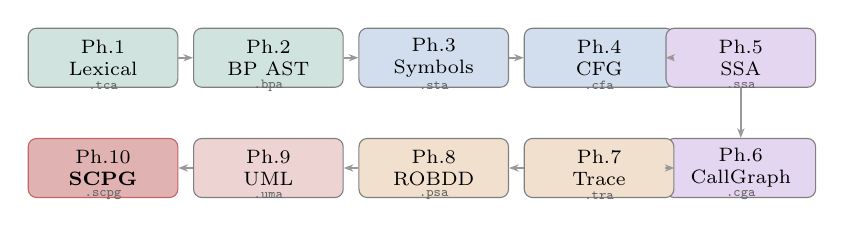
\begin{tikzpicture}[
  ph/.style={
    draw=black!50, rounded corners=3pt,
    minimum width=1.9cm, minimum height=0.75cm,
    font=\scriptsize, align=center, inner sep=2pt
  },
  art/.style={font=\tiny\ttfamily, text=black!60},
  a/.style={-{Stealth[length=3.5pt]},thick,black!40}
]
% Row 1
\node[ph,fill=colA!20] (p1) at (0,2.2)
  {Ph.1\\Lexical};
\node[ph,fill=colA!20] (p2) at (2.1,2.2)
  {Ph.2\\BP AST};
\node[ph,fill=colB!20] (p3) at (4.2,2.2)
  {Ph.3\\Symbols};
\node[ph,fill=colB!20] (p4) at (6.3,2.2)
  {Ph.4\\CFG};
\node[ph,fill=colC!20] (p5) at (8.1,2.2)
  {Ph.5\\SSA};

\node[art] at (0,1.85) {.tca};
\node[art] at (2.1,1.85) {.bpa};
\node[art] at (4.2,1.85) {.sta};
\node[art] at (6.3,1.85) {.cfa};
\node[art] at (8.1,1.85) {.ssa};

% Row 2
\node[ph,fill=colC!20] (p6) at (8.1,0.8)
  {Ph.6\\CallGraph};
\node[ph,fill=colD!20] (p7) at (6.3,0.8)
  {Ph.7\\Trace};
\node[ph,fill=colD!20] (p8) at (4.2,0.8)
  {Ph.8\\ROBDD};
\node[ph,fill=colE!20] (p9) at (2.1,0.8)
  {Ph.9\\UML};
\node[ph,fill=colE!35,draw=colE!70] (p10) at (0,0.8)
  {Ph.10\\\textbf{SCPG}};

\node[art] at (8.1,0.45) {.cga};
\node[art] at (6.3,0.45) {.tra};
\node[art] at (4.2,0.45) {.psa};
\node[art] at (2.1,0.45) {.uma};
\node[art] at (0,0.45) {.scpg};

% Row 1 arrows
\draw[a] (p1.east)--(p2.west);
\draw[a] (p2.east)--(p3.west);
\draw[a] (p3.east)--(p4.west);
\draw[a] (p4.east)--(p5.west);
% Turn
\draw[a] (p5.south)--(p6.north);
% Row 2 arrows
\draw[a] (p6.west)--(p7.east);
\draw[a] (p7.west)--(p8.east);
\draw[a] (p8.west)--(p9.east);
\draw[a] (p9.west)--(p10.east);
\end{tikzpicture}
\caption{Data flow between OpenHeart's ten pipeline phases.
Each phase reads all prior artifacts and emits one new
immutable artifact.  Phase~10 merges all nine artifacts into
the unified \texttt{.scpg} binary.}
\label{fig:pipeline}
\end{figure}

\subsection{Phases 1--2: From Source to Succinct AST}

\textbf{Phase~1} parses each source file with a
language adapter~\cite{treesitter}, assigns monotonically
increasing \textit{token identifiers}, interns all text
via FNV-1a hashing, and sorts the resulting token records
by sort key (Equation~\ref{eq:sortkey}).

\textbf{Phase~2} reduces the parse tree to an AST via
language-specific rules (\textsc{Keep} / \textsc{Eliminate}
/ \textsc{Drop}), encodes the result as a BP string,
and builds the jump table $\mathit{jt}[2n_a]$ in
$\BigO(n_a)$ by a single stack sweep (Algorithm~\ref{alg:jt}).
Token ranges are propagated bottom-up: leaf nodes inherit
their own token identifier; internal nodes take the min and
max of their children's ranges.

\begin{algorithm}[t]
\caption{Jump Table Construction (Phase~2)}
\label{alg:jt}
\small
\begin{algorithmic}[1]
\Require BP string $B \in \{0,1\}^{2n}$
\Ensure $\mathit{jt}[i]$ = matching parenthesis of $B[i]$
\State $\mathit{stk} \gets []$
\For{$i \gets 0$ \textbf{to} $2n-1$}
  \If{$B[i] = 1$}
    \State $\mathit{stk}.\mathrm{push}(i)$
  \Else
    \State $o \gets \mathit{stk}.\mathrm{pop}()$;\;
      $\mathit{jt}[o] \gets i$;\; $\mathit{jt}[i] \gets o$
  \EndIf
\EndFor
\end{algorithmic}
\end{algorithm}

From the BP string, rank-select index, and jump table, all
standard tree navigation operations run in $\BigO(1)$:
\begin{alignat}{2}
  &\mathrm{first\_child}(v)
    &&= \rank_1(\pre(v)+1)-1
    \quad\text{if }B[\pre(v)+1]=1\notag\\
  &\mathrm{next\_sibling}(v)
    &&= \rank_1(\mathit{jt}[\pre(v)]+1)-1\notag\\
  &\mathrm{parent}(v)
    &&= \rank_1(\mathrm{enc}(\pre(v)))-1\notag\\
  &\mathrm{subtree\_size}(v)
    &&= (\mathit{jt}[\pre(v)]-\pre(v)+1)/2\notag
\end{alignat}

\subsection{Phases 3--6: Semantic and Interprocedural Analysis}

\textbf{Phase~3} builds the symbol table $\VSYM$ and type
hierarchy $\ETH$ via five passes over the BP AST.  Name
resolution uses scope graphs~\cite{antwerpen16}, a
language-agnostic formalism that models nested scopes as a
graph and resolves names by BFS.  Multiple passes are
structurally necessary (not a design choice) because Java
and similar languages permit forward references.

\textbf{Phase~4} constructs per-function CFGs by recursive
descent and computes immediate dominators using the
iterative algorithm of Cooper et al.~\cite{cooper01}
(convergence guaranteed by the RPO traversal order).
Dominance frontiers---required by Phase~5 for
$\phi$-placement---follow from the idom array in
$\BigO(|E_f| \cdot \mathrm{depth})$ per function.

\textbf{Phase~5} converts each function to SSA form via the
two-pass Cytron algorithm~\cite{cytron91}: first,
$\phi$-functions are placed at iterated dominance frontiers
(Algorithm~\ref{alg:phi}); then variables are renamed by DFS
over the dominator tree.  Three IFDS analyses follow on the
resulting SSA/CDG structure: taint propagation, nullable
pointer analysis, and type-state analysis.

\begin{algorithm}[t]
\caption{$\phi$-Function Placement~\cite{cytron91}}
\label{alg:phi}
\small
\begin{algorithmic}[1]
\ForAll{variable $v$}
  \State $W \gets \mathrm{defsites}(v)$;\; $P \gets \emptyset$
  \While{$W \ne \emptyset$}
    \State $b \gets W.\mathrm{pop}()$
    \ForAll{$y \in \DF[b]$}
      \If{$y \notin P$ \textbf{and} $v \in \mathrm{LiveIn}(y)$}
        \State insert $\phi_y(v)$;\;
          $P \gets P \cup \{y\}$
        \If{$y \notin \mathrm{defsites}(v)$}
          \State $W \gets W \cup \{y\}$
        \EndIf
      \EndIf
    \EndFor
  \EndWhile
\EndFor
\end{algorithmic}
\end{algorithm}

\textbf{Phase~6} extracts call sites from the BP AST and
resolves targets via Class Hierarchy Analysis
(CHA)~\cite{lhotak03}, refined by SSA-based 1-CFA
(if the receiver is defined by \texttt{new\;T()}, the
target set is exactly $\{T.m\}$) and Anderson's
inclusion-based points-to analysis~\cite{anderson94}.
Tarjan's algorithm~\cite{tarjan72} identifies recursive
SCCs in $\BigO(|V|+|E|)$.

\subsection{Phases 7--10: Synthesis and Assembly}

\textbf{Phase~7} materializes $\tauF$ for all six entity
layers, builds the Symbol Span Index $\FI$, and pre-computes
UMLLink records for all UML-relevant symbols.  The SCPG
hash chain (Equation~\ref{eq:hashchain}) is computed here.

\textbf{Phase~8} constructs $\ROBDD(f_{\mathrm{paths}})$
for each function by: computing an initial variable ordering
via FORCE~\cite{aloul03} on the constraint hypergraph; building
the ROBDD by conjoining structural flow-conservation clauses
via the BDD \textsc{Apply} operation~\cite{bryant86}; and
refining the ordering by Rudell's sifting~\cite{rudell93}.
Functions are processed in SCC condensation-DAG order so
that callee summaries are available when callers are built.

\textbf{Phase~9} applies extraction functions to produce
UML metadata for all fourteen diagram types (Table~\ref{tab:uml}).
CFG blocks map to UML activity node types: binary-branching
blocks become \textit{DecisionNodes}; join points become
\textit{MergeNodes}; straight-line blocks become
\textit{ActionNodes}.  State machines are extracted from
IFDS type-state pairs grouped by class type.

\textbf{Phase~10} merges all nine artifacts into a unified
memory-mapped binary with eleven typed sections ordered by
access frequency (hot $\to$ warm $\to$ cold).  The uncompressed
size is ${\sim}305\,\mathrm{MB}$, compressing to
${\sim}82\,\mathrm{MB}$ with LZ4.  A demand-driven query
engine with a 512-entry LRU cache (keyed by query type,
parameter hash, and $\hscpg$) is bootstrapped on the
completed binary.

% ============================================================
\section{Theoretical Guarantees}\label{sec:theory}

\subsection{Space Efficiency (R1)}

We first state the two foundational results whose combination
yields the SCPG's space bound.

\begin{theorem}[BP Space; Munro and Raman~\cite{munroraman97}]
\label{thm:bp}
An ordered forest on $n$ nodes can be stored in
$2n + o(n)$ bits, with all of
$\{\mathrm{first\_child},\mathrm{next\_sibling},\mathrm{parent},
\mathrm{subtree\_size},\mathrm{depth},\mathrm{LCA}\}$
answerable in $\BigO(1)$ time.
\end{theorem}

\begin{proof}
The information-theoretic lower bound is $2n - \BigO(\log n)$
bits (by the Catalan count $C_n \sim 4^n / n^{3/2}$ distinct
forests).  The BP encoding achieves exactly $2n$ bits,
matching within $\BigO(\log n)$.  A Jacobson~\cite{jacobson89}
rank-select index of size $\BigO(n/\log n)$ words supports
$\rank_1$ and $\sel_1$ in $\BigO(1)$.  The navigation
formulas for all listed operations follow from
$\rank_1$, $\sel_1$, and the jump table $\mathit{jt}$;
LCA reduces to Range-Minimum on the excess
sequence~\cite{benderfarach00} in $\BigO(1)$.
\end{proof}

\begin{theorem}[Wavelet Tree; Grossi et al.~\cite{grossi03}]
\label{thm:wt}
A sequence of length $m$ over alphabet $\Sigma$ with
$|\Sigma| = \sigma$ can be stored in
$m\lceil\log_2\sigma\rceil + \BigO(m)$ bits supporting
access, rank, and select in $\BigO(\log\sigma)$, and
type-filtered enumeration in $\BigO(\log\sigma)$ per element.
\end{theorem}

\begin{proof}
Standard; see Grossi et al.~\cite{grossi03}.  The wavelet
tree has $\lceil\log_2\sigma\rceil$ levels, each an $m$-bit
bitmap with rank-select index; each query traverses the
root-to-leaf path in $\BigO(\log\sigma)$ steps.
\end{proof}

Combining these with the SSA $\phi$-function count
(Cytron et al.~\cite{cytron91}: $\BigO(|E_{\mathrm{cfg}}|)$
per function) and the ROBDD bound of the next subsection,
we obtain:

\begin{theorem}[SCPG Space Complexity]\label{thm:space}
The SCPG can be stored in
$\BigO(n_a + m\lceil\log_2\sigma\rceil + n_s + n_t +
\textstyle\sum_f |\ROBDD(f)|)$ bits plus $\BigO(n)$ machine
words of auxiliary index structure, where $n_a = |\VS \cup \VT|$,
$m = |E|$, $n_s = |\VSYM|$, $n_t = |\VT|$.  For structured
programs and $\sigma \le 256$, this is $\BigO(n\log\sigma)$
$= \BigO(8n)$ bits.
\end{theorem}

\begin{proof}[Proof sketch]
Token layer: $128n_t$ bits (16-byte records).
AST layer (Theorem~\ref{thm:bp}): $\BigO(n_a)$ bits.
Graph layers (Theorem~\ref{thm:wt}): $\BigO(m\log\sigma)$
bits per CSR+WT structure; $\BigO(m\log\sigma)$ summed.
SSA/DFG layer: $\BigO(n_a)$ machine words by
Lemma~\ref{lem:ssasparse}.
Symbol layer: $512n_s$ bits (64-byte records).
Traceability layer: $\BigO(n)$ machine words (dense arrays).
Path summaries: $96\sum_f|\ROBDD(f)|$ bits; for SP programs,
$\sum_f|\ROBDD(f)| = \BigO(m)$ by Theorem~\ref{thm:robdd}.
Summing yields $\BigO(n\log\sigma)$.
\end{proof}

\subsection{Auxiliary Lemmas}

The following four lemmas are required stepping stones for
the traceability and ROBDD theorems.  Each addresses a
distinct structural property of the SCPG's components.

\begin{lemma}[Sort Key Uniqueness]\label{lem:sortkey}
$\sortkey(t_i) \ne \sortkey(t_j)$ for any two distinct
tokens $t_i, t_j$.
\end{lemma}

\begin{proof}
Any scanner produces at most one token starting at each
character offset, so distinct tokens have distinct
$(\mathit{file}, \ell, c)$ triples.
Equation~\eqref{eq:sortkey} is injective because
the three fields occupy non-overlapping bit ranges
($16 + 24 + 16 = 56 \le 64$ bits) within their respective
bounds.
\end{proof}

\begin{lemma}[BP Bijectivity]\label{lem:bpbij}
$v \mapsto \pre(v)$ is a bijection between AST nodes and
$1$-bit positions in $\mathrm{BP}(F_{\mathrm{ast}})$.
\end{lemma}

\begin{proof}
Each node contributes exactly one $1$-bit at $\pre(v)$; the
DFS visits each node once, so the map is injective.
The number of $1$-bits equals $n_a$, so it is also surjective
onto the set of $1$-bit positions.
\end{proof}

\begin{lemma}[Dominance Frontier Cardinality]\label{lem:dfcard}
$\sum_{b \in B_f} |\DF(b)| \le |E_f|$.
\end{lemma}

\begin{proof}
Each CFG edge $(p, y)$ can contribute $y$ to $\DF(b)$ for
at most one $b$ (the deepest dominator of $p$ that does not
strictly dominate $y$).  Hence the total count of
$(b,y)$ pairs is at most $|E_f|$.
\end{proof}

\begin{lemma}[SSA Def-Use Sparsity]\label{lem:ssasparse}
The total number of SSA def-use edges is
$\BigO(|E_{\mathrm{cfg}}|)$.
\end{lemma}

\begin{proof}
By Lemma~\ref{lem:dfcard}, total $\phi$-insertions are
$\BigO(|E_{\mathrm{cfg}}|)$.  Ordinary definitions number at
most $n_a$.  Since $|E_{\mathrm{cfg}}| \ge n_a - 1$ in any
connected CFG, all terms are $\BigO(|E_{\mathrm{cfg}}|)$.
\end{proof}

\subsection{Path Summaries (R4, partial)}

The key structural result is that for programs without
\texttt{goto}, the ROBDD encoding of the feasible path set
is polynomial in the number of CFG edges.

\begin{definition}[Series-Parallel CFG]\label{def:sp}
A CFG $G_f$ is \emph{series-parallel} (SP) iff constructible
from a single edge by repeated \emph{series composition}
(appending one SP graph to another) or \emph{parallel
composition} (sharing entry and exit of two SP graphs).
Every structured program free of \texttt{goto} has an SP
CFG~\cite{valdes79}.
\end{definition}

\begin{definition}[Feasible Path Function]\label{def:pathfunc}
For $G_f$ with $m$ edges, assign variable $x_e$ to edge $e$.
The \emph{feasible path function}
$f_{\mathrm{paths}} : \{0,1\}^m \to \{0,1\}$ equals $1$
iff the assignment $(x_e)_{e \in E_f}$ encodes a
structurally consistent path from entry to exit.
For a block $b$ with predecessors $p_1,\ldots,p_k$ and
successors $s_1, s_2$ (binary branch):
\begin{equation}\label{eq:phib}
  \Phi_b = \Bigl(\bigvee_j x_{p_j \to b}\Bigr)
  \to (x_{b \to s_1} \oplus x_{b \to s_2}).
\end{equation}
Then $f_{\mathrm{paths}} = \bigwedge_b \Phi_b \wedge
C_{\mathrm{entry}} \wedge C_{\mathrm{exit}}$.
\end{definition}

\begin{theorem}[ROBDD Size for SP CFGs]\label{thm:robdd}
For any SP CFG with $m$ edges, there exists a variable
ordering $\pi$ such that
$|\ROBDD_\pi(f_{\mathrm{paths}})| \le 2m - 1$.
\end{theorem}

\begin{proof}
By structural induction on the SP decomposition.

\smallskip\noindent\emph{Base case.}
A single edge $e$ with variable $x_e$.
$\ROBDD(x_e)$ has one internal node (var $= x_e$,
$\mathrm{lo} = \mathbf{0}$, $\mathrm{hi} = \mathbf{1}$).
$|\ROBDD| = 1 = 2(1) - 1$. \cmark

\smallskip\noindent\emph{Series.} $G_f = G_1 \cdot G_2$
with disjoint edge sets $X_1, X_2$ and $|X_i| = m_i$.
Order all $X_1$ variables before $X_2$.
Then $f_{\mathrm{paths}} = f_1(X_1) \wedge f_2(X_2)$.
In the ROBDD, the $X_1$ subtree equals $\ROBDD(f_1)$;
each $\mathbf{1}$-leaf is replaced by the root of
$\ROBDD(f_2)$, which is shared (Reduction Rule~R2) across
all such leaves.  Hence:
\[
  |\ROBDD(f_1 \wedge f_2)|
  \le |\ROBDD(f_1)| + |\ROBDD(f_2)|
  \le (2m_1\!-\!1) + (2m_2\!-\!1)
  \le 2m - 1.
\]

\smallskip\noindent\emph{Parallel.} $G_f = G_1 \parallel G_2$
with fork variables $x_\ell, x_r$.
Order $x_\ell < x_r < \pi_1 < \pi_2$.
Then $f_{\mathrm{paths}} = (x_\ell \wedge f_1) \vee
(x_r \wedge f_2)$.
The root node splits on $x_\ell$; its lo-branch leads to
$f_2$ (since $x_r = 1$) and its hi-branch to $f_1$.  Both
subtrees are stored once by Rule~R2:
\[
  |\ROBDD| \le 1 + |\ROBDD(f_1)| + |\ROBDD(f_2)|
  \le 2m - 1.
\]
By induction the bound holds for all SP CFGs.
\end{proof}

\begin{corollary}[$\SATC$ in Linear Time]\label{cor:sat}
The total number of feasible execution paths through $f$ is
computable in $\BigO(|\ROBDD(f)|)$ by a memoized DFS:
\[
  \mathrm{count}(N) = 2^{g_0}\!\cdot\!\mathrm{count}(\mathrm{lo}(N))
  + 2^{g_1}\!\cdot\!\mathrm{count}(\mathrm{hi}(N))
\]
where $g_i$ is the variable-index gap to the $i$-th child.
\end{corollary}

\subsection{Traceability Completeness (R2)}

\begin{theorem}[Traceability Completeness]\label{thm:trace}
Let $\SCPG$ be an OpenHeart SCPG.  Then:
\begin{enumerate}
\item[\emph{(i)}] $\tauF$ is total: $\tauF(\varepsilon)$
  is well-defined for every $\varepsilon \in \mathcal{E}$.
\item[\emph{(ii)}] $\forall\, t \in \VT$:
  $(L_0, t) \in \tauI(\tauF(L_0,t))$.
\item[\emph{(iii)}] $\forall\, (\ell, \mathit{id})$:
  $(\ell, \mathit{id}) \in \tauI(\tauF(\ell,\mathit{id}))$.
\end{enumerate}
\end{theorem}

\begin{proof}
\emph{(i) Totality.}
Every $t \in \VT$ has a valid $\BI[t]$ (Phase~1 assigns a
$\BI$ entry to every token; Invariant: $\forall t$,
$\BI[t].\mathit{token\_id} = t$).  By Phase~2's bottom-up
range sweep, every AST node has valid $\mathit{ft}(v) \le
\mathit{lt}(v)$.  Higher-layer equations
(\ref{eq:tau2})--(\ref{eq:tau5}) delegate to lower layers;
SSA $\phi$-functions (which have no direct definition
statement) fall back to $\tauF(L_3, \mathit{def\_block}(v))$,
which is valid by Phase~4's block metadata construction.

\emph{(ii) Token roundtrip.}
Phase~7 inserts a Symbol Span Index record for every
$t \in \VT$ with $\mathit{ft} = \mathit{lt} = t$.
The stabbing condition $\mathit{ft} \le t \le \mathit{lt}$
is satisfied with equality, so $(L_0, t) \in \tauI(t)$.

\emph{(iii) Higher-layer roundtrip.}
For $(\ell, \mathit{id})$ with range
$[\mathit{ft}_R, \mathit{lt}_R]$, Phase~7 inserts a $\FI$
record with these exact bounds.  For $t = \mathit{ft}_R$, the
stabbing condition holds, so $(\ell, \mathit{id})
\in \tauI(t) = \tauI(\tauF(\ell,\mathit{id}))$.
\end{proof}

\subsection{Dataflow and Path Queries (R4)}

\begin{theorem}[IFDS; Reps et al.~\cite{reps95}]\label{thm:ifds}
Any IFDS problem with distributive flow functions over
a program with $|N|$ nodes and fact set $D$ is solvable
in $\BigO(|N| \cdot |D|^2)$ time via path-edge tabulation.
\end{theorem}

\begin{proof}
Distributivity ($f(X \cup Y) = f(X) \cup f(Y)$) enables
path merging at join points without loss of precision.
The tabulation algorithm of Reps et al.~\cite{reps95}
propagates path edges $(n_1,d_1) \leadsto (n_2,d_2)$ across
the exploded supergraph $G^\# = N \times (D \cup \{\perp\})$;
each of at most $|N|^2 \cdot |D|^2$ edges is inserted once.
With memoization, total work is $\BigO(|N| \cdot |D|^2)$.
\end{proof}

\begin{theorem}[CFL-Reachability; Reps~\cite{reps97}]
\label{thm:cfl}
Interprocedural path queries on the call supergraph $G^*$
are answerable in $\BigO(|V_{\mathrm{CG}}|^3)$ via cubic
tabulation.
\end{theorem}

\begin{proof}
By reduction to CFL-reachability for the Dyck language
over $G^*$~\cite{reps97}.  The algorithm maintains summary
edges $(s,e)$; each of at most $|V|^2$ pairs is processed
in $\BigO(|V|)$, giving $\BigO(|V|^3)$.
\end{proof}

\subsection{Incremental Updates}

\begin{theorem}[Incremental Update Complexity]\label{thm:incr}
Let $\Delta$ be a source edit affecting only the body
of function $f$.  The SCPG update cost is:
\[
  T(\Delta) = \BigO\!\left(n_{s,f}\log n_{s,f}
    + n_{b,f}^2 + n_{\mathrm{ssa},f}|D|^2
    + m_f\,|\ROBDD(f)|\right)
\]
where all quantities are local to $f$.
\end{theorem}

\begin{proof}
A body-only edit leaves the symbol table and call graph
topology unchanged (function signature is unmodified).
Only $f$'s body is re-processed: Phase~1 re-sorts $f$'s
tokens ($\BigO(n_{s,f}\log n_{s,f})$); Phase~4 recomputes
$f$'s CFG and dominators ($\BigO(n_{b,f}^2)$ by Cooper's
algorithm~\cite{cooper01}); Phase~5 runs SSA and IFDS on
$f$ ($\BigO(n_{\mathrm{ssa},f}|D|^2)$); Phase~8 rebuilds
$\ROBDD(f)$ ($\BigO(m_f|\ROBDD(f)|)$).  No other function
is reanalyzed.
\end{proof}

\subsection{UML Completeness (R3)}

\begin{table}[!t]
\renewcommand{\arraystretch}{1.2}
\caption{All 14 UML Diagram Types and Their SCPG Source}
\label{tab:uml}
\centering
\small
\begin{tabular}{@{}l@{\;}l@{\;}l@{}}
\toprule
\textbf{Diagram} & \textbf{Type} & \textbf{SCPG Source}\\
\midrule
Class          & Structural & $\VSYM + \ETH$\\
Object         & Structural & SSA allocation sites\\
Component      & Structural & Packages $+ \ECG$\\
Deployment     & Structural & Module annotations\\
Package        & Structural & Namespace hierarchy\\
Composite Str. & Structural & Inner class structure\\
Profile        & Structural & Annotation type decls\\
Use Case       & Behavioral & $\ECG$ fan-in$=0$ methods\\
Activity       & Behavioral & $\VB + \ECFG + \SigPhi$\\
State Machine  & Behavioral & IFDS type-state\\
Sequence       & Behavioral & $\ECG$ call sites\\
Communication  & Behavioral & $\ECG$ + TRA spans\\
Interaction Ov.& Behavioral & Activity + Sequence\\
Timing         & Behavioral & Thread analysis\\
\bottomrule
\end{tabular}
\end{table}

\begin{corollary}[All 14 UML Diagrams in Polynomial Time]
\label{cor:uml}
Each diagram type in Table~\ref{tab:uml} is extractable
from the SCPG in time polynomial in $n = |V| + |E|$.
\end{corollary}

\begin{proof}
Structural diagrams scan $\VSYM + \ETH$ in $\BigO(n_s + m)$.
Activity diagram traverses the CFG in $\BigO(n_{b,f}+m_f)$
and reads ROBDD metrics in $\BigO(1)$.
State machine enumerates IFDS type-state pairs in
$\BigO(n_{\mathrm{ssa}}|D|)$.
Sequence is DFS over $\ECG$ in
$\BigO(|V_{\mathrm{CG}}|+|E_{\mathrm{CG}}|)$.
Use Case scans $\VSYM$ for fan-in-zero public methods in
$\BigO(n_s)$.  Remaining diagrams are derived views; all
bounds are polynomial.
\end{proof}

% ============================================================
\section{The Query Engine}\label{sec:query}

The query engine operates as a demand-driven layer over the
memory-mapped SCPG binary.  Queries are dispatched against
the appropriate section of the binary and memoized in an
LRU cache of capacity 512 entries.  The cache is keyed by
$(q_{\mathrm{type}}, h_{\mathrm{params}}, \hscpg)$;
an $\hscpg$ mismatch (caused by a source edit) triggers
lazy invalidation---no cache scan is needed, only a stored
hash write---since entries with the old hash silently fail
their hash comparison at next access.

Table~\ref{tab:querycmplx} lists all primary query types
with their first-run complexity and the SCPG binary sections
they access.  Navigation queries are the hot path in IDE
integration and run in $\BigO(1)$/$\BigO(\log n)$; diagram
generation runs in time linear in the output size; and
CFL-reachability, though cubic in theory, is sub-second for
$|V_{\mathrm{CG}}| \le 15{,}000$ due to the early-termination
structure of the tabulation.

\begin{table}[!t]
\renewcommand{\arraystretch}{1.2}
\caption{Query Complexity (cached queries: $\BigO(1)$)}
\label{tab:querycmplx}
\centering
\small
\begin{tabular}{@{}lll@{}}
\toprule
\textbf{Query} & \textbf{First Run}
  & \textbf{Sections}\\
\midrule
$\tauF(\varepsilon)$ (navigate to source)
  & $\BigO(1)$ & $\BI$ (0x09)\\
$\tauI(\mathit{file},t)$ (navigate from source)
  & $\BigO(\log n_s + k)$ & $\FI$ (0x09)\\
Class diagram
  & $\BigO(n_s)$ & 0x04, 0x08, 0x0A\\
Activity diagram ($f$)
  & $\BigO(n_{b,f}+m_f)$ & 0x05, 0x0B, 0x0A\\
Sequence diagram
  & $\BigO(|V|+|E|)_{\mathrm{CG}}$ & 0x07, 0x0A\\
$\mathrm{isReachable}(s,t)$
  & $\BigO(|V_{\mathrm{CG}}|^2)$ & 0x07\\
Backward slice (depth $d$)
  & $\BigO(n_{\mathrm{ssa}} d)$ & 0x06, 0x07\\
Path count ($f$)
  & $\BigO(1)$ & 0x0B metrics\\
Test coverage
  & $\BigO(|\ROBDD|+|\mathrm{traces}|)$ & 0x0B\\
\bottomrule
\end{tabular}
\end{table}

% ============================================================
\section{Formal Comparison with Prior Work}\label{sec:comparison}

\begin{proposition}\label{prop:prior}
The following violations hold:
CPG/Joern~\cite{yamaguchi14} violates \emph{R1}, \emph{R2},
and \emph{R3}.
LLVM IR~\cite{lattner04} violates \emph{R2} and \emph{R3}.
EMF/XMI~\cite{emf} violates \emph{R1}, \emph{R2},
and \emph{R4}.
WALA~\cite{wala} violates \emph{R1} and \emph{R3}.
\end{proposition}

\begin{proof}
\textbf{CPG, R1.}  OverflowDB relationship records cost
$34\;\mathrm{bytes}$ each~\cite{yamaguchi14}, versus
SCPG's $(4 + \lceil\log_2 16\rceil / 8)\cdot m \le 4.5m$
bytes for $\sigma = 16$: a factor-of-$7.5$ violation.

\textbf{CPG, R2.}  Source locations in Joern are property
pairs on AST nodes with no bijective token-level forward
index and no formal roundtrip guarantee
(Theorem~\ref{thm:trace} does not hold for CPG).

\textbf{CPG, R3.}  The CPG has no ROBDD path summaries,
no IFDS type-state analysis, and no UML extraction layer.
Activity, state machine, and timing diagrams cannot be
derived from CPG without additional components outside
the CPG specification.

\textbf{LLVM IR, R2.}  DWARF DILocation attaches to LLVM
instructions, not source tokens~\cite{lattner04}.
Multi-expression statements map all derived instructions
to a single line number; column-level traceability is not
part of the IR specification.

\textbf{LLVM IR, R3.}  Virtual dispatch is lowered to
\texttt{getelementptr} + indirect call, irreversibly
discarding class hierarchy information.  UML class diagram
generation requires language-specific reverse engineering
with no completeness guarantee.

\textbf{EMF/XMI, R1.}  Each attribute name-value pair
serializes as $\ge 10$ bytes of XML markup~\cite{emf}.
A class with 5 methods and 10 attributes produces
$\sim 1{,}050$ bytes versus the SCPG's 64-byte
SymbolRecord---a $16\times$ overhead.

\textbf{EMF/XMI, R4.}  EMF/XMI is a serialization format;
all queries require full deserialization to an in-memory
object graph before any analysis can begin.

\textbf{WALA, R1.}  JVM object overhead per analysis
artifact is $120$--$200\;\mathrm{bytes}$ versus the SCPG's
16-byte SSARecord.

\textbf{WALA, R3.}  WALA has no UML generation capability;
its output is Java data structures requiring a separate
transformation pipeline.
\end{proof}

% ============================================================
\section{Limitations and Discussion}\label{sec:limits}

\paragraph{ROBDD Worst Case.}
Theorem~\ref{thm:robdd} applies to series-parallel CFGs.
Production code sometimes contains exception-handler
nesting or state-machine-style \texttt{goto} patterns
(e.g., in the Linux kernel or Android AOSP) that violate
the SP property, potentially causing exponential ROBDD
growth.  We mitigate this with bounded unwinding
($k \le 3$ levels) using the $\BigO(n)$ SP-recognition
algorithm of Valdes et al.~\cite{valdes79}, producing a
sound under-approximation.

\paragraph{Points-To Precision.}
Anderson's analysis~\cite{anderson94} is flow-insensitive
and heap-insensitive.  Frameworks that use runtime
dependency injection (Spring Boot, Android's Binder IPC)
may produce false call-graph edges that cannot be pruned
without runtime information.  Such sites are conservatively
tagged as \textsc{CG\_Reflection} and excluded from
CFL-reachability while remaining in the call graph for
structural diagram generation.

\paragraph{Multi-Language Boundaries.}
Call edges crossing language boundaries (Java/JNI,
Python/Cython) cannot be statically resolved.  Each boundary
generates a conservative external stub symbol, preserving
soundness within each language while acknowledging the gap.

\paragraph{Hash Collision Probability.}
CRC-64 is not cryptographically collision-resistant.
For detecting accidental staleness after normal edits,
it is sufficient.  Deployments requiring tamper-evidence
should substitute SHA-256 at higher computation cost.

% ============================================================
\section{Related Work}\label{sec:related}

The CPG of Yamaguchi et al.~\cite{yamaguchi14} is the
closest prior work and the primary baseline for this paper.
It unifies AST, CFG, and PDG in a property graph and has
enabled significant advances in vulnerability
detection~\cite{yamaguchi14}.  As shown in
Section~\ref{sec:comparison}, however, it violates R1--R3.
The SCPG is conceptually a successor that replaces the
property graph backend with succinct representations, adds
the SSA, IFDS, and ROBDD layers, and provides a formal
traceability guarantee.

LLVM IR~\cite{lattner04} and MLIR~\cite{lattner21} are the
standard compiler IRs.  They are designed for optimization
and code generation, not visualization; their lowering
pipeline is designed to be semantics-preserving but
structure-discarding.  The SCPG explicitly keeps all
high-level structure intact, making it a complement to
rather than a replacement for these IRs.

Static analysis frameworks including WALA~\cite{wala} and
Soot~\cite{lhotak03} provide rich interprocedural analyses
but do not guarantee the space bounds of R1 or the
traceability guarantee of R2.

Abstract interpretation~\cite{cousotcousot77} provides the
theoretical underpinning for the IFDS analyses in Phase~5.
Scope graphs~\cite{antwerpen16} provide the name-resolution
formalism used in Phase~3.

% ============================================================
\section{Conclusion}\label{sec:concl}

We have presented the Succinct Compositional Program Graph
and the OpenHeart pipeline, establishing that a single
data structure can simultaneously satisfy all four
requirements---space efficiency, absolute traceability,
UML semantic completeness, and polynomial query
complexity---that a universal program representation must
meet.

The central technical contributions are: a novel structural
induction proof that ROBDD path summaries for structured
programs have size $\BigO(m)$ (Theorem~\ref{thm:robdd}),
not requiring treewidth machinery; a formal completeness
proof for the bidirectional traceability function
(Theorem~\ref{thm:trace}); and the $\BigO(|\Delta|)$
incremental update result (Theorem~\ref{thm:incr}) that
makes OpenHeart viable as the analysis backend for an
interactive IDE.

Future work includes a full implementation with empirical
evaluation on industrial codebases; extension of
Theorem~\ref{thm:robdd} to non-SP CFGs via treewidth
decompositions~\cite{bodlaender98}; and whole-program
ROBDD path queries via compositional call-summary encoding.

\bibliographystyle{IEEEtran}
\bibliography{openheart}

\end{document}
